%%%%%%%%%%%%%%%%%%%%%%%%%%%%%%%%%%%%%%%%%%%%%%%%%%%%%%%%%%%%%%%%%%%%%%%%%%%%%%%%
%2345678901234567890123456789012345678901234567890123456789012345678901234567890
%        1         2         3         4         5         6         7         8

\documentclass[letterpaper, 10 pt, conference]{ieeeconf}  % Comment this line out if you need a4paper

%\documentclass[a4paper, 10pt, conference]{ieeeconf}      % Use this line for a4 paper

\IEEEoverridecommandlockouts                              % This command is only needed if 
                                                          % you want to use the \thanks command

\overrideIEEEmargins                                      % Needed to meet printer requirements.

%In case you encounter the following error:
%Error 1010 The PDF file may be corrupt (unable to open PDF file) OR
%Error 1000 An error occurred while parsing a contents stream. Unable to analyze the PDF file.
%This is a known problem with pdfLaTeX conversion filter. The file cannot be opened with acrobat reader
%Please use one of the alternatives below to circumvent this error by uncommenting one or the other
%\pdfobjcompresslevel=0
%\pdfminorversion=4

% See the \addtolength command later in the file to balance the column lengths
% on the last page of the document

% The following packages can be found on http:\\www.ctan.org
%\usepackage{graphics} % for pdf, bitmapped graphics files
%\usepackage{epsfig} % for postscript graphics files
%\usepackage{mathptmx} % assumes new font selection scheme installed
%\usepackage{times} % assumes new font selection scheme installed
%\usepackage{amsmath} % assumes amsmath package installed
%\usepackage{amssymb}  % assumes amsmath package installed
\hyphenation{op-tical net-works semi-conduc-tor}

\usepackage[]{graphicx} % added to make your file compilable
\usepackage{subfigure}
\usepackage{fixltx2e}
\usepackage{refstyle}
\usepackage{float}
\usepackage{multicol}
\usepackage{multirow}
\usepackage{booktabs}
\usepackage{diagbox}
\usepackage{tabularx}
\usepackage{fancyhdr}
\usepackage{fancyhdr}
\usepackage{amsmath}
\usepackage{algorithm}    
\usepackage{algorithmicx}
\usepackage{algpseudocode}
\usepackage{amssymb}
\usepackage{bm}
%\usepackage{flushend}

\def\RSfigtxt{Fig.\,}%
\def\RSfigstxt{Figs~}%
\def\RSFigtxt{Fig.\,}%
\def\RSFigstxt{Figs~}%
\def\keywordsname{Keywords}

\floatname{algorithm}{Algorithm}
\renewcommand{\algorithmicrequire}{\textbf{Input:}}
\renewcommand{\algorithmicensure}{\textbf{Output:}}

\title{\huge \bf
Fast adaptive control of snake robots for pole climbing\vspace{1.7mm}
}


\author{
\authorblockN{Zhiyong Jian\authorrefmark{1}, Jianping Huang\authorrefmark{1}, Yuhong Huang\authorrefmark{2}, Linlin Liu\authorrefmark{1}, Long Cheng\authorrefmark{1} and Kai Huang\authorrefmark{1}}
\authorblockA{\authorrefmark{1}School of Data and Computer Science,Sun yat-sen University, Guangzhou, China \\ Email: jianzhy5@mail2.sysu.edu.cn} 
\authorblockA{\authorrefmark{1}Email: huangjp25@mail2.sysu.edu.cn} 
\authorblockA{\authorrefmark{1}Email: liull28@mail2.sysu.edu.cn} 
\authorblockA{\authorrefmark{2}College of Computer, National University of Defense Technology, ChangSha, China \\Email: huangyuhong17@nudt.edu.cn}
\authorblockA{\authorrefmark{1}Email: chengl@in.tum.de} 
\authorblockA{\authorrefmark{1}Email: huangk36@mail.sysu.edu.cn}  
}


\begin{document}


\maketitle
\thispagestyle{empty}
\pagestyle{empty}


%%%%%%%%%%%%%%%%%%%%%%%%%%%%%%%%%%%%%%%%%%%%%%%%%%%%%%%%%%%%%%%%%%%%%%%%%%%%%%%%
\begin{abstract}

Snake-liked robots are a class of biomorphic hyper-redundant robots
consist of many chain-connected active joint modules. Autonomy of this
kind of robots is however a complex problem. This paper proposes an
adaptive control framework for the pole climbing of snake robots. By
clustering the unsupervised training data and fast multi-parameter
regression, our framework can rapidly react to environment
changes. Experimental results show that, by using our framework, the
overhead of choosing new control parameters is about 100\,ms and our
snake robot can climb poles with different diameters.
\end{abstract}

\begin{keywords}
Snake-liked robots; autonomous ability; pipe climbing; weighted regression; machine learning
\end{keywords}


%%%%%%%%%%%%%%%%%%%%%%%%%%%%%%%%%%%%%%%%%%%%%%%%%%%%%%%%%%%%%%%%%%%%%%%%%%%%%%%%
\section{Introduction}
% no \IEEEPARstart
%Snake-like robots generally consist of rigid links connected by joints which are usually fitted with actuators to control the locomoton to form a serial structure that mimic the skeleton of a real snake. With multiple joints and degree of freedom, snake-like robots have strong mobility in complex and unknown terrains\cite{Chirikjian1995The}. Therefore, they can complete tasks in many occasions, such as disaster rescuing\cite{DogAndSnake}, factory pipe maintenance\cite{ACMTutorial} and scientific exploration\cite{Kuwada2007Snake}. In the past decades, with the advent of orthogonal and universal joint structure\cite{1014757}\cite{Date2005Control}\cite{GaitBasedCompliant},  snake-like robots acquired the ability of three-dimensional space movement, which strengthens their mobility in varied topography. 

%Although the snake-like robots have high mobility in many environments, the control of snake-like robots is complicated. A variety of motions can be constructed to get the same motion effect in the same environment because of the features of snake-like robots like multiple joints and degree of freedom. Moreover, the movements of snake-like robots are difficult to be predicted in the unknown environment.

%Nowadays, there are two widely used control method. Firstly, we can pre-define the parameters to make robots move correctly in the known environment based on a widely used motion model\cite{HiroseSine} of snake-like robots. However, this method is not feasible for the unknown environment. Secondly, we can control the robot by tunning parameters artificially. While tunning parameters artifically is inefficient in unknown environments because it is difficult to tune the parameter accurately during robots' motion. In addition, controlling the robots is a professional work and tunning the parameters inaccurately will break the motion of snake-like robots. Therefore, autonomous mobility of robots is an expectation in robots' motion.
%Although the snake-like robots have high mobility in many environments, the movement of most snake-like robots in unknown environments is directly controlled by human, reducing the efficiency and limiting the implementation of snake-like robots. Therefore, it is an important and challenging task to give them the ability to move in complex environment without real-time human intervention, that is, the autonomous mobility.

%Autonomous mobility is an important and challenging task in robots' controlling.  Autonomous mobility requires high real-time performance to make robots respond to changes in the environment in time. What's more, High efficiency is critical in autonomous mobility. With high real-time performance and high efficiency, robots can make a rapid calculation when a mutation happens in the motion environment .   

%In this paper, we propose a novel experience-based control strategy, which autonomously determines the optimal control parameters of a snake-like robot in current environment by entropy variance\cite{WaveformEntropyVariance}\cite{EntropyandVarianceasRiskMeasure}\cite{UsingEntropyAndVariance}. By tunning the optimal control parameter with regression value through the weighted least squares algorithm\cite{gradientMethod}\cite{MSEestimates}, we achieve to make the robot gradually adapt itselt to the environment. The whole process of our control strategy can be divided into two parts:
%\begin{enumerate}
%	\item data acquisition and preprocessing,
%	\item real-time data feedback and multi-parameter regression control.
%\end{enumerate}
%\begin{figure}[!t]
%	\centering
%	\subfigure[Reality robot]{
%		\includegraphics[width=1.5in,height=0.75in]{fig/relative/realSnake}
%		\figlabel{fig:snake_like_robot_a}
%	}
%	\subfigure[Simulation robot]{
%		\includegraphics[width=1.5in,height=0.75in]{fig/relative/simulateSnake}
%		\figlabel{fig:snake_like_robot_b}
%	}
%	\caption{The Snake-like robot}
%	\figlabel{fig:snake_like_robot}
%\end{figure}
%In the first part, we collect data that reflecting the dynamic states of a snake-like robot in varies environments and then form a training set. The clustering algorithm\cite{Cluseter_ICT}\cite{KmeansAndDeepLearning} is adopted in this part to reduce the time overhead of feed-back control. In the second part, we apply regression and feed-back control based on previous training data of the motion of robots. The multi-parameter regression is also transformed into an unit regression problem for higher efficiency. We adopt the entropy variance\cite{WaveformEntropyVariance}\cite{EntropyandVarianceasRiskMeasure}\cite{UsingEntropyAndVariance} as the criterion for accessing the effect of the control parameters on the motion. Then the most sensitive parameter which has the greatest effect on motion is selected to perform the unit regression. By transforming the multiple regression into the  unit regression and combining the weighted least squares algorithm\cite{gradientMethod}\cite{MSEestimates},  we finally get a fitted regression function and obtain the value of the optimal parameter.
%To evaluate the effectiveness of the proposed framework, we also apply it to the our existing snake-like robot platform, which is shown in~\figref{fig:snake_like_robot_a} and~\figref{fig:snake_like_robot_b}. Under our framework, the robot climbs pipes having different diameters and the performance of climbing is reported. In summary, the contributions of this paper are: 
%\begin{itemize}
%	\item A new framework for robot adaptive control is proposed.
% 	      This framework greatly reduces the amount of  effort of the regression calculation 
%           by adopting clustering algorithm for data preprocessing and the classification of 
%           real-time data.
%	\item A transformation of multiple regression problem is proposed to obtain the optimal
%          control parameters in a real-time manner.
%         The entropy variance is utilized to select the parameter which is the most sensitive 
%         in current state. Then, by regressing this parameter instead of all the parameters, the 
%         multiple regression is transformed into an unit regression problem.
%    \item A set of case studies is conducted and the results demonstrate
%    that our proposed strategy is effectiveness in accomplishing autonomous movement for snake-like robots.
%\end{itemize}
%The robot has an orthogonal structure with 18 joints. Each joint has a rotation axis which
%is perpendicular to the body. The rotation axes of two adjacent joints are orthogonal with each other,
%thus forming a three-dimensional space movement. a set of sensors such as accelerometer and gyro
%is embedded in each joint to realize the feedback control.

%The rest of this paper is organised as follows. Early preparations are demonstrated in the Section \uppercase\expandafter{\romannumeral2}. In Section \uppercase\expandafter{\romannumeral3}, proposed strategy is explained in detailed. And then Simulation works are illustrated in Section \uppercase\expandafter{\romannumeral4}. Section \uppercase\expandafter{\romannumeral5} shows the conclusion and our future prospects about the proposed strategy.

%The simulation environment is the pipe climbing, which can be used in cable detection of cable-stayed bridge. In the first part, we collect data in pipes with different diameter as training set. To reduce time of calculation in feed-back control, we adopt clustering algorithm\cite{Cluseter_ICT}\cite{KmeansAndDeepLearning}. In the second part, we apply regression and feed-back control based on previous training data on the motion of robots. We utilize the entropy variance\cite{WaveformEntropyVariance}\cite{EntropyandVarianceasRiskMeasure}\cite{UsingEntropyAndVariance} to measure the effect of the control parameters on the motion and select the most sensitive parameter which has the greatest effect on motion. By transforming the multiple regression into the unit regression and combining the weighted least squares algorithm\cite{gradientMethod}\cite{MSEestimates}, we finally get a fitted regression function and modify the most sensitive parameter.

Snake robots are a class of biomorphic hyper-redundant
robots~\cite{Chirikjian1995The}, designed to imitate the snake
creatures’ biological limbless locomotion with outstanding rapidity,
stability, and diversity in wild environment. Typically, these
snake robots consist of many chain-connected active joint
modules, giving them kinematic versatility, like bending, stretching,
and crispation.  A considerable number of these robots have been
implemented in various fields, such as disaster rescuing, factory
maintenance, and terrorism surveillance.

In order to better complete predefined tasks, snake robots are
required to obtain capabilities of moving autonomously and behaving
self-adaptively~\cite{Liljeb2013Snake}, e.g., making decision when,
where, and how to move based on different situations of itself and
environment. Automatically adapting to the environment is, however,
not easy. The reasons are multi-folds. First, due to the redundant
degrees of freedom, the locomotion of the snake robot is
difficult to model, especially including the complex interaction
between the robot and the environment.  The corresponding control for
this multi-degree locomotion is even more complicate. Second, when
encountering an environment which is not known beforehand, how to
decide a suitable control strategy is obvious. Even for a given
control strategy, how to decide its parameters is not
straightforward. Third, the runtime procedure of deciding the control
strategy and its corresponding parameters must be efficient, i.e., in
real time. Otherwise, the desired locomotion of the robot will most
probably fail.

To let the robots adapt to an unknown environment, methods that use
the sensors to perceive the environment and to embed the environment
perception rules has been widely
used~\cite{CPGenabling,GaitBasedCompliant,BalancingAndControl,FeedbackControlOfSoft}. Tang
et al. proposed a control strategy based on CPG(central pattern
generator) model~\cite{CPGenabling}. Rollinson et al. proposed a
snake robot adaptive control based on state
estimation~\cite{GaitBasedCompliant}.  As the model in these methods is
a gradient model based on state estimation, these they are not suited
to the mutation environment.
There are researchers that have proposed neural network models
combined with physical environment information to determine the
control
scheme~\cite{InformationDriven,NovelPlasticityRule,MissileSystems,NeuroFuzzyBayesian}. These
models are only the control suggestion and may not make a good effect
on real-time motion of the robots.

In this paper, a new framework for adaptive control of snake robots is
proposed. Based on data that are collected off-line by unsupervised
training, our framework can efficiently adapt new control parameters
for environment changes by fast regression. Specifically, we target
pole climbing, which demands a fast response to the environment
changes. In this scenario, if the control cannot adapt on-time, the
robot will fall.  To evaluate the effectiveness of the proposed
approach, we conduct experiments on a snake robot on different
poles. The experimental results show that the overhead of runtime
adaptation is slightly more than 100\,ms and snake robot can fast
adapt to different poles and climb along the poles smoothly. The
contributions of this paper are:
\begin{itemize}
\item A adaptive control framework for the pole climbing of snake
  robots. For the offline unsupervised training, a k-means++ method is
  used to cluster the collected data. During runtime, the Z-axis
  velocity of the robot is used as a feed-back signal to continuously
  adapt new control parameters of the robot.
\item A transformation of multiple regression problem is proposed to
  obtain the optimal control parameters in a real-time manner.  The
  entropy variance is utilized to select the parameter which is the
  most sensitive in current state. Then, by regressing this parameter
  instead of all the parameters, the multiple regression is
  transformed into an unit regression problem.
\item A set of case studies is conducted and the results demonstrate
  that our proposed strategy is effectiveness in accomplishing
  autonomous movement for snake robots.
\end{itemize}

The rest of this paper is organised as follows. The relative work is shown in Section \uppercase\expandafter{\romannumeral2} and an overview of our work is
demonstrated in the Section \uppercase\expandafter{\romannumeral3}. In
Section \uppercase\expandafter{\romannumeral4} and \uppercase\expandafter{\romannumeral5}, proposed strategy is
explained in detailed. And then Simulation works are illustrated in
Section \uppercase\expandafter{\romannumeral6}. Section
\uppercase\expandafter{\romannumeral7} shows the conclusion and our
future prospects about the proposed strategy.
%\section{Relative work}
Our existing snake-liked robot platform is shown in~\figref{fig:snake_like_robot_a}. The joints of snake-liked robots are connected orthogonally. We also build the simulation snake-liked robot(~\figref{fig:snake_like_robot_b}) and embeded a set of sensors like angle sensors and distance sensors to realize the feedback control of robots.
\begin{figure}[!t]
	\centering
	\subfigure[Reality robot]{
		\includegraphics[width=1.5in,height=0.75in]{fig/relative/realSnake}
		\figlabel{fig:snake_like_robot_a}
	}
	\subfigure[Simulation robot]{
		\includegraphics[width=1.5in,height=0.75in]{fig/relative/simulateSnake}
		\figlabel{fig:snake_like_robot_b}
	}
	\caption{The Snake-liked robot}
	\figlabel{fig:snake_like_robot}
\end{figure}

Currently, a widely used of control strategy for snake-liked robots is based on the sinusoidal motion model\cite{HiroseSine} which is proposed by professor Hirose. After that, Tesch et al. proposed a parametric equation based on the sinusoidal model for a snake-liked robot with three-dimensional athleticism\cite{ChosetSine}. This parametric equation simplifies the control strategy of the snake-like robots and allows the robot to determine the movement model of the machine with a small amount of control parameters. In order to ensure that snake-like robots can be applied to a wider scene, robots need to have autonomous mobility in the unknown and complex environment. Therefore, we propose a control strategy by experience-based learning combined with clustering~\cite{Cluseter_ICT,KmeansAndDeepLearning} and weighted regression.

%To make the robots adapt to the unknown environment, the method which use the sensors to perceive the environment and embed the environment perception rules, has been widely used\cite{CPGenabling}\cite{GaitBasedCompliant}\cite{BalancingAndControl}\cite{FeedbackControlOfSoft}. Tang et al. proposed a control strategy based on CPG(central pattern generator) model\cite{CPGenabling}. Rollinson et al. proposed a snake-like robot adaptive control based on state estimation\cite{GaitBasedCompliant}. However, a complete correlation prediction model of control parameters is not given in their paper. As their methods is a gradient model based on state estimation, thus they are not suited to the mutation environment. What's more, there are researchers that have proposed a neural network model combined with physical environment information to determine the control scheme\cite{InformationDriven}\cite{NovelPlasticityRule}\cite{MissileSystems}\cite{NeuroFuzzyBayesian}. This model is only the control suggestion and may not make a good effect on motion in real-time motion of the robot. 
%To make the robots adapt to the unknown environment, the method which use the sensors to perceive the environment and embed the environment perception rules, has been widely used\cite{CPGenabling}\cite{GaitBasedCompliant}\cite{BalancingAndControl}\cite{FeedbackControlOfSoft}. Tang et al. proposed a control strategy based on CPG(central pattern generator) model\cite{CPGenabling}. Rollinson et al. proposed a snake-like robot adaptive control based on state estimation\cite{GaitBasedCompliant}. However, a complete correlation prediction model of control parameters is not given in their paper. As their methods is a gradient model based on state estimation, they are not suited to the mutation environment.
%To adapt to the environment, the method which use the sensors to perceive the environment and embed the environment perception rules, has been widely used\cite{CPGenabling}\cite{GaitBasedCompliant}\cite{BalancingAndControl}\cite{FeedbackControlOfSoft}. Tang et al. proposed a control strategy based on CPG(central pattern generator) model\cite{CPGenabling}. They achieve to control the gait change to adapt to the environment by taking speed as a measure,  embedding several gaits to the robots and combining with CPG control according to the environment. Rollinson et al. proposed a snake-like robot adaptive control based on state estimation\cite{GaitBasedCompliant}. A complete correlation prediction model of control parameters is not given in their paper. As it is based on state estimation, this method is a step-by-step change model, thus it is not suited to the mutation environment. %There are some algorithms of machine learning in the robot control applications\cite{InformationDriven}\cite{NovelPlasticityRule}\cite{MissileSystems}\cite{NeuroFuzzyBayesian}. They only give control program conversion but do not provide changes in the control strategy.

%On the application of machine learning in the field of robot control, there are researchers that have proposed a neural network model combined with physical environment information to determine the control scheme\cite{InformationDriven}\cite{NovelPlasticityRule}\cite{MissileSystems}\cite{NeuroFuzzyBayesian}. This model is only the control suggestion and may not make a good effect on motion in real-time motion of the robot. 

%In this paper, a control strategy by experience-based learning  is proposed. Combined with the clustering\cite{Cluseter_ICT}\cite{KmeansAndDeepLearning} and the multi-parameter regression, we realize the real-time autonomous change of multiple control parameters in the robots' movement.

\section{Overview}
Our approach proposed in this paper is shown in \figref{fig:stepMap}. We divide our approach into two main parts: off-line work and runtime execution.
\begin{figure}[H]
	\centering
	\includegraphics[width=1.0\linewidth,height=140pt]{fig/mainwork/stepMap}
	\caption{The overall approach}
	\figlabel{fig:stepMap}
\end{figure}

In off-line work, firstly, we define parameter space and let the robot climb the poles with different diameters by different parameters which are stable during climbing. When the robot are climbing the pole, we record the velocity and joint angles of the robot every two seconds. After that, we combine all the data from climbing different poles together and then conduct clustering~\cite{Cluseter_ICT,KmeansAndDeepLearning} on the whole data.

In runtime execution, we will collect the real-time data like joint angles,  velocity and the value of parameters every two seconds and then select the  data recorded in off-line work to our calculation by clustering the real-time data. After selecting the data we need, we determine the parameter whose change has the greatest effect on the motion of the robot by entropy variance. And finally we get the new value of the selected parameter by weighted regression. 

Currently, a widely used of control strategy for snake-liked robots is based on the sinusoidal motion model~\cite{HiroseSine} which is proposed by professor Hirose. After that, Tesch et al. proposed a parametric equation based on the sinusoidal model for a snake-liked robot with three-dimensional athleticism~\cite{ChosetSine}. This parametric equation simplifies the control strategy of the snake-like robots and allows the robot to determine the motion model of the machine with a small amount of control parameters. We take rolling gait~\cite{Enner2013Motion} as our climbing gait in simulation. The sinusoidal motion model function about rolling gait is shown in the following formula:
\begin{eqnarray}\label{basicRoll}
T_i=\left\{
\begin{array}{lr}
A\cdot \sin (\omega \cdot t + i\cdot \varepsilon )&odd\\
A\cdot \sin (\omega \cdot t + i\cdot \varepsilon +  \frac{\pi}{2})&even
\end{array}
\right.
\end{eqnarray}

By modifying the amplitude $A$, phase $\varepsilon$, and angular rate $\omega$ in Eq.\ref{basicRoll}, the maximum rotation angle of joints, robots' shape and the motion rate of the snake-liked robot are changed. Unlike the biological snake, rolling gait can be performed by snake-liked robot. Rolling gait is an easy but effective gait. Snake-liked robot can move on the ground or climb the pole by rolling gait with suitable parameters.

%\section{experience-based control strategy}
\section{off-line work}

%\begin{figure}[H]
%	\centering
%	\includegraphics[width=.8\linewidth]{fig/mainwork/stepMap}
%	\caption{The overall experimental flow chart}
%	\figlabel{fig:stepMap}
%\end{figure}

In the preprocessing work, we let the robot move along 25\,cm and 35\,cm poles for a large number of times and we collect and store the data listed in the form like Table \ref{dataTable}.
%\begin{figure}[H]
%	\centering
%	\includegraphics[width=\linewidth]{fig/mainwork/data}
%	\caption{The structure of the data storage}
%	\figlabel{fig:data}
%\end{figure}
\begin{table}[h]
    \begin{center}
        \caption{recorded value during training}
        \label{dataTable}
        \begin{tabular}{cl cl} 
            \toprule
            \multicolumn{1}{m{3cm}}{\centering Symbol}
            &\multicolumn{1}{m{4cm}}
              {\centering Definition}\\
            \midrule
			\multirow{2}{*}{$\theta_{m,i}$} & The joint angle of the $i_{th}$ joint which is\\& measured \\
			\multirow{2}{*}{$M$} & \multirow{2}{*}{Mean of the measured joint angles} \\
			\multirow{2}{*}{$\upsilon_{z}$} & \multirow{2}{*}{The Z-axis velocity} \\\\	\hline
			\multirow{2}{*}{$A$} & \multirow{2}{*}{The value of amplitude} \\
			\multirow{2}{*}{$\omega$} & \multirow{2}{*}{The value of angular rate} \\
			\multirow{2}{*}{$\varepsilon$} & \multirow{2}{*}{The value of phase} \\\\
            \bottomrule
        \end{tabular}
    \end{center}
\end{table}

We define $M$ as $\frac{\sum_{i=1}^{n}\theta_{m,i}}{n} $ where n is the number of joints. $\theta_{m}=\begin{bmatrix}
\theta_{m,1} & \theta_{m,2} & \cdots & \theta_{m,n}
\end{bmatrix}$ is the joint angles which are measured. The control vector is shown as
$\begin{bmatrix}
A& \omega&\varepsilon
\end{bmatrix}$
where $A$ is the amplitude, $\omega$ is the angular rate, and the $\varepsilon$ is the phase. All of them are applied in Eq.\ref{basicRoll}.

After collecting movement data of a snake-liked robot, we combine the training data obtained in different environment and then cluster the data in order to optimize real-time calculation.

%\subsection{Implementation of Clustering by $k-means++$}
In this research, collected data in preprocessing is a large-scale data set. As k-means++ algorithm has high efficiency and scalability for a large-scale data set, we adopt $kmeans++$ for clustering. We classify training set into $N$ clusters. The clustering process is divided into the following steps:
\begin{itemize}
	\item Step 1: Decide the value of $N$ by Eq.\ref{clu_var}.
	\begin{eqnarray}\label{clu_var}
		N=arg\min \limits_{N_{k}}{\frac{\sum _{N_{k}}(S_{i}-E)^{2}}{N_{k}}}
	\end{eqnarray}
	where $E = \frac{\sum _{N}(S_{i})}{N}$ and $i\in [1,N]$.
	\item Step 2: perform k-means++ as \textbf{Algorithm \ref{kmeans}} shows. K-means++ is an improvement on the k-means algorithm. By function INITIALIZE, we can obtain $N$ initial cluster centers. And then, we iterate function UPDATE to update the cluster centers and the clusters until the cluster centers do not change any more.
%	\item Step 2: Randomly select a point in the training set as the first cluster center.
%	\item Step 3: For the $k_{th}$ center, select the point which has the largest  distance to the $(k-1)$ centers in the current training set
	%prework step2
%	\begin{eqnarray}\label{clu_step2}
%	\left\{
%	\begin{array}{lr}
%	F_{c}\left ( P^{\left (  i\right )} \right ) = \sum_{j=1}^{k-1}\left \| X^{\left ( j-1 \right )}-P^{\left (  i\right )} \right \|_{2}\\
%	k = $arg$\max \limits_{i}{(F_{C}(P^{(i)}))}
%	\end{array}
%	\right.
%	\end{eqnarray}
%	\begin{figure}[H]
%		\centering
%		\includegraphics[height=0.5in]{fig/mainwork/data2}
%		\caption{Data vector used in clustering and regression}
%		\figlabel{fig:data2}
%	\end{figure}
%	$P^{(i)}$ is $\begin{bmatrix}
%	\theta_{m} & M
%	\end{bmatrix}$. $X^{(j)}$ is the $j_{th}$ cluster center. $S^{(P)}$ is the  training set. For the initial cluster center $X^{(k)}$, we have $X^{(k)}\in S^{(P)}$ and $X^{(k)}$ is the vector $P^{(i)}$ which corresponds to the result of Eq.\ref{clu_step2}. 
%	\item Step 4: Repeat Step 1 and Step 2 until $N_{k}$ cluster centers have been confirmed.
%	\item Step 5: After confirming $N_{k}$ cluster center, we categorize every vector in training set based on Eq.\ref{clu_step4}.
	%prework step4
%	\begin{eqnarray}\label{clu_step4}
%	C^{(i)} = arg\min \limits_{k}{(||P^{(i)}-X^{(k)}||_{2})}
%	\end{eqnarray}
%	In this equation, $C^{(i)}$ is the flag of category which the vector $P^{(i)}$ belongs to.
%	\item Step 6: Refresh the cluster centers according to clustering result by the Eq.\ref{clu_step5}
	%prework step5
%	\begin{eqnarray}\label{clu_step5}
%	X^{(k)}=\frac{\sum_{i}\{C^{(i)}=k)\}P^{(i)}}{\sum_{i}\{C^{(i)}=k\}}
%	\end{eqnarray}
%	\item Step 7: iterate Step 4 and 5 until the cluster centers change within a predefined tolerance range.
\end{itemize}

\begin{algorithm}
    \caption{k-means++}
    \label{kmeans}
    \begin{algorithmic}[1] 
       \Require Training set $\bm{P}$, The number of clusters $N$
       \Ensure Set of cluster centers $\bm{X}$
       \Function {Initialize}{$\bm{P}, N$}
           \State $\bm{X} \gets sample \ a \ point \ randomly \ from \ \bm{P}$
           \While{$\vert \bm{X} \vert<N$}
               \For{$i = 1 \to \vert \bm{P} \vert$}
                   \State $I \gets arg\min \limits_{i}\left({\sum_{j=1}^{\vert \bm{X} \vert} {\Vert X_j - P_i \Vert}^2  }\right)$
                   \State $\bm{X} \gets \bm{X} \cup \left\{ P_I \right\}$
                   \State $\bm{P} \gets \bm{P} - P_I$
               \EndFor
           \EndWhile
           \State \Return{$\bm{X}$}
       \EndFunction
       \State
       \Function{Update}{$\bm{P}, \bm{X}$}
           \While{$\textbf{X}$ does not change any more}
               \For{$i = 1 \to \vert \bm{P} \vert$}
      \State $C_i \gets arg\min \limits_{k}{\left( {\Vert P_i - X_k\Vert} ^2\right)}$
               \EndFor
               \For{$k = 1 \to \vert \bm{X} \vert$}
      \State $X_k \gets \frac{\sum_{i}{\left\{C_i=k\right\}P_i}}{\sum_{i}{\left\{C_i=k\right\}}}$
               \EndFor
           \EndWhile
           \State \Return{$\bm{X}$}
       \EndFunction
\end{algorithmic}
\end{algorithm}

With $Kmeans++$, the collected data can be divided into $N$ clusters. After finishing the clustering, the result is stored in two parts:

\begin{enumerate}
	\item The cluster centers $\textbf{X}$.
	\item The member $P_{i},i \in [1,\vert \bm{P} \vert]$ of the cluster center $X_{k},k \in [1,N]$
\end{enumerate}

\section{runtime}
In robot's running time, we get the real-time data periodically and then we do the following steps. Firstly, we categorize the real-time data based on the clustering result in off-line work. And then we select the most sensitive gait parameter according to the entropy variance. At last, we use the idea of weighted regression to modify the selected gait parameter and keep the other gait parameters unchanged.
\subsection{Parameter selection by entropy variance}

%classification
\subsubsection{Real-time data categorization}

Every time we get the real-time data, we relegate it to the certain cluster by Eq.\ref{cluster}.
\begin{eqnarray}\label{cluster}
C=arg\min \limits_{k}{(||X_{k}-P_{t}||_{2})} \, ,&X_{C}\in \bm{X}
\end{eqnarray}

$\bm{X}$ is the cluster center set(\textbf{Algorithm \ref{kmeans}}). $X_{C}$ is the closet center to the real-time data vector $P_t$. And $X_{k}$ is the $k_{th}$ cluster center of the cluster center set $\bm{X}$ . With $Euclidian \; Distance \; Formula$, we make a prediction on the similarity between two data vectors.

\subsubsection{The selection of the preponderant data}

After categorization of real-time data, we select those preponderant vectors whose Z-axis velocity are bigger than current (Eq.\ref{preponderant}).
%find out preponderant
\begin{eqnarray}\label{preponderant}
\bm{P_{\upsilon}}=\{P_{i} | \upsilon_{z,i}\geq \upsilon_{z,P_{t}} \; , \; P_{i}\in \bm{P_{C}}\}
\end{eqnarray}

$\bm{P_{C}}$ is all the data vectors which belong to the cluster with the  center $X_{C}$. $\upsilon_{z,i}$ is the vertical velocity component of the data vector $P_{i}$ and $\upsilon_{z,P_{t}}$ is the vertical velocity component of the real-time data vector. $\bm{P_{\upsilon}}$ is the set of all the preponderant vectors for regression.

\subsubsection{The selection of the sensitive parameter}

We adopt entropy variance as the reference to select the parameter which should be modified. The steps of selecting the sensitive parameter are as follows.

\begin{itemize}
	\item Step 1: We take the preprocessing operation to discrete the preponderant data (Eq.\ref{quantification}).
	%quantification
	\begin{eqnarray}\label{quantification}
	\upsilon_{new,i}=\left\{
	\begin{array}{lr}
	\left \lfloor \frac{\upsilon_{z,i}}{L_{D}} \right \rfloor&\upsilon_{z,i}> 0\\
	\\
	\left \lceil \frac{\upsilon_{z,i}-L_{D}}{L_{D}} \right \rceil&\upsilon_{z,i}\leq 0
	\end{array}
	\right.
	\end{eqnarray}
	
	In Eq.\ref{quantification}, $L_{D}$ is the adjustable step length for discretization. We eventually get the velocity discrete sequence:
	\begin{eqnarray}\label{newMember}
	V_{new}=\begin{bmatrix}
	\upsilon_{new,1} & \upsilon_{new,2} & \upsilon_{new,3} & \upsilon_{new,4} & \cdots & \cdots
	\end{bmatrix}
	\end{eqnarray}
	
	\item Step 2: There are a variety of possible values for each gait parameter. Thus, in order to record all the possible values, we make a set $S_{i,j}$ with the gait parameter $i$'s value is its $j_{th}$ possible value. And the value of $i$ is from 0 to 2 representing $A$, $\omega$ and $\varepsilon$ respectively. We calculate the entropy about the vertical velocity when the gait parameter $i$'s value is its $j_{th}$ possible value by Eq.\ref{entropy} as well as the entropy variance of the gait parameter $i$ by Eq.\ref{var_entropy}. In Eq.\ref{entropy}, $p(\upsilon_{new,k})$ is the appearance rate of the $V_{i,j}$ in $S_{i,j}$. In Eq.\ref{var_entropy}, $E_{i,j}$ is the mean of velocity when the gait parameter $i$'s value is its $j_{th}$ possible value. And $N_{i}$ is the number of possible values of the gait parameter $i$.
	%entropy
	\begin{eqnarray}\label{entropy}
	H(S_{i,j})=-\sum _{\upsilon_{new,k}\in V_{new}}p(\upsilon_{new,k})log_{2}p(\upsilon_{new,k})
	\end{eqnarray}
	
	%entropy variance
	\begin{eqnarray}\label{var_entropy}
	Var_{i}=\frac{\sum _{N_{i}}(H(S_{i,j})-E_{i,j})^{2}}{N_{i}}
	\end{eqnarray}
	
	\item Step 3: We normalize the entropy variance (Eq.\ref{normalize}) and randomly select the sensitive gait parameters by Roulette wheel selection algorithm. %(\figref{fig:Roulette}) to avoid the selection getting stuck in the high probability event.
	%normalize entropy variance
	\begin{eqnarray}\label{normalize}
	R_{Var_{i}}=\frac{Var_{i}}{\sum Var_{i}}
	\end{eqnarray}
	
	%\begin{figure}[H]
	%	\centering
	%	\includegraphics[width=\linewidth]{fig/mainwork/Roulette}
	%	\caption{Sensitive parameter selection by roulette method}
	%	\figlabel{fig:Roulette}
	%\end{figure}
\end{itemize}

After the calculation of gait parameters' entropy variance. the sensitive parameter will be found. And then the selected parameter's value will be modified by regression.


\subsection{Assignment to the value of the selected parameter}

In this research, we take weighted regression to get the value of the sensitive gait parameter and use the gradient descent method to solve the weighted least squares problem in fitting regression function.

\begin{itemize}
	\item Step 1: List the fitting prediction function(Eq.\ref{fitfunction})
	%fitting and estimation function
	\begin{eqnarray}\label{fitfunction}
	F_{w}(P_{t})=W^{T}P_{t}\,,&W=\begin{bmatrix}w_{1}\\ w_{2}\\ \vdots \\ w_{m}\end{bmatrix}
	\end{eqnarray}
	
	In Eq.\ref{fitfunction}, $W$ is the coefficient sequence of the fitting equation and $m$ is the number of coefficients where $P_{t}$ is the real-time collected data vector. Then we can get the error function(Eq.\ref{estimate}) which takes the square of error as the estimation with $n$ being the number of data of $\bm{P_{\upsilon}}$ and $\bm{Q}$ being the set consisting of the value of selected parameter in $P_{i}$.
	%Square sum as an estimation
	\begin{eqnarray}\label{estimate}
		D(W)=\frac{1}{2n}(F_{w}(\bm{P_{\upsilon}})^{T}-\bm{Q})^{T}(F_{w}(\bm{P_{\upsilon}})^{T}-\bm{Q})
	\end{eqnarray}
	\begin{eqnarray}
		\bm{P_{\upsilon}}=\begin{bmatrix}P_{\upsilon,1}&P_{\upsilon,2}  &\cdots  &P_{\upsilon,n} \end{bmatrix}
	\end{eqnarray}
	\begin{eqnarray}
		\bm{Q}=\begin{bmatrix}Q_{\upsilon,1}& Q_{\upsilon,2}& \cdots & Q_{\upsilon,n}\end{bmatrix}^{T}
	\end{eqnarray}
	
	To get the best-fit coefficient sequence $W$ by the minimum $D(w)$, according to gradient descent method, we turn the Eq.\ref{estimate} into Eq.\ref{Gradde}.
	%Gradient descent
	\begin{eqnarray}\label{Gradde}
	\nabla_{w}D=\frac{1}{n}\bm{P_{\upsilon}}(F_{w}(\bm{P_{\upsilon}})^{T}-\bm{Q})
	\end{eqnarray}
	
	\item Step 2: Perform the weighted operation on preponderant data vector to ensure the estimate result of fitting is good (Eq.\ref{WeiGradde}).
	%weighted gradient
	\begin{eqnarray}
	\nabla_{w}D=\frac{1}{n}\bm{P_{\upsilon}}M(F_{w}(\bm{P_{\upsilon}})^{T}-\bm{Q})
	\end{eqnarray}
	\begin{eqnarray}\label{WeiGradde}
	M=\begin{bmatrix}
	\frac{\upsilon_{z,1}}{L_{s}}&0&\cdots&0\\
	0&\frac{\upsilon_{z,2}}{L_{s}}&\ddots&0\\
	\vdots&\ddots&\ddots&0\\
	0&\cdots&0&\frac{\upsilon_{z,3}}{L_{s}}
	\end{bmatrix}
	\end{eqnarray}
	In Eq.\ref{WeiGradde}, $L_s$ is the learning step and $M$ is the learning rate matrix.
	
	\item Step 3: Fit the coefficient vector by Eq.\ref{fit}.
	%fitting the parameters
	\begin{eqnarray}\label{fit}
	W=W-\nabla_{w}D
	\end{eqnarray}
	In this way, the coefficient sequence $W$ is updated.
	
	\item Step 4: Iterate the steps above until we acquire the best-fit coefficient. The value of $W$ is stable finally.
\end{itemize}

When the iteration is stopped, the best-fit coefficient $W_{best}$ will be obtained. By applying $W_{best}$ to Eq.\ref{result}, we can get the regression value of the sensitive parameter. This value will be used in the robot control. It is worth noting that we only modify the sensitive parameter and others remain the same value.
%compensation result
\begin{eqnarray}\label{result}
Q_{t} = F_{w}(P_{t})=W^{T}P_{t}
\end{eqnarray}
%\input{complexity}
\section{SIMULATION}
We use the rolling gait as the basic gait for simulations. To verify the adaptability of snake-liked robots under our proposed adaptive control, we conduct simulations on poles with different diameters under the robot simulation platform V-REP.

The simulation process can be divided into two categories: training and motion simulation. And we divide simulations into two parts: the adaptable motion along poles having changing diameter and the adaptable motion along straight poles with different diameters.

\subsection{Training process}

In the data acquisition process, we let the robot climb along the 25\,cm and 35\,cm poles under different parameters and collect 25 thousand volumes of training data in total. The interval of amplitude $A$, phase $\varepsilon$ and angular rate $\omega$ are $[40, \, 80]$, $[0, \, 5]$ and $[1.5, \, 3]$ respectively. What's more, the step of $A$ is 5, the step of $\varepsilon$ is 1 and the step of $\omega$ is 0.5. We make the robot climb poles with different combination of parameters and then collect the data. In the preprocessing process, we cluster the training data. We set the number of clusters as 25 by Eq.\ref{clu_var} and \figref{fig:clusize}. The number of data for most of classes is $1000 \pm 500 $ (\figref{fig:clustersize}).

\begin{figure}[!h]
	\centering
	\includegraphics[width=1.0\linewidth,height=125pt]{fig/experiment/170912/clusize}
	\caption{The variance in cluster size of $N_{k}$}
	\figlabel{fig:clusize}
\end{figure}

\begin{figure}[t]
	\centering
	\includegraphics[width=0.8\linewidth]{fig/experiment/170912/cluster}
	\caption{The result of clustering}
	\figlabel{fig:clustersize}
\end{figure}

\subsection{the autonomous motions along a variable diameter pole}

\begin{figure}[!h]
	\centering
	\subfigure[t=24s]{
		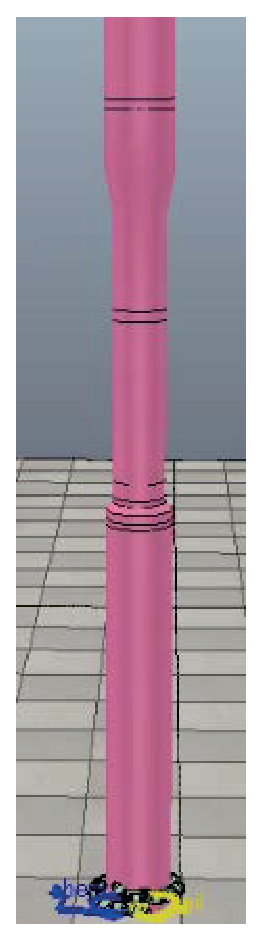
\includegraphics[height=2in,width=.12\textwidth]{fig/experiment/BSB/34s}
	}
	\subfigure[t=35s]{
		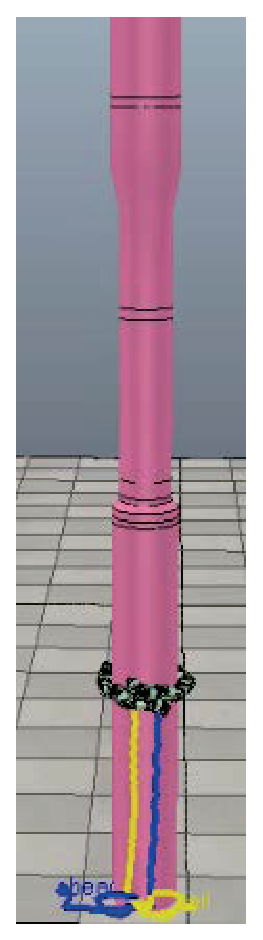
\includegraphics[height=2in,width=.12\textwidth]{fig/experiment/BSB/49s}
	}
	\subfigure[t=47s]{
		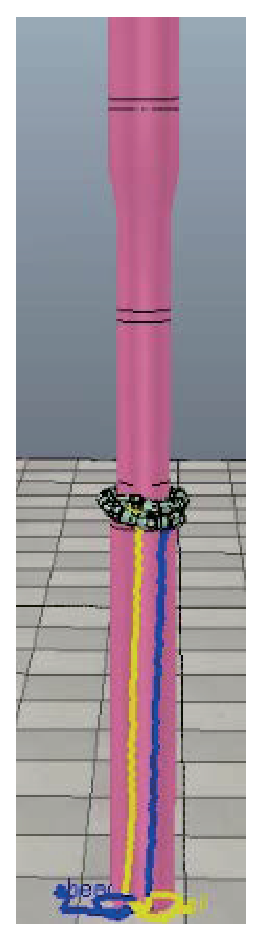
\includegraphics[height=2in,width=.12\textwidth]{fig/experiment/BSB/1m05s}
	}
	\subfigure[t=56s]{
		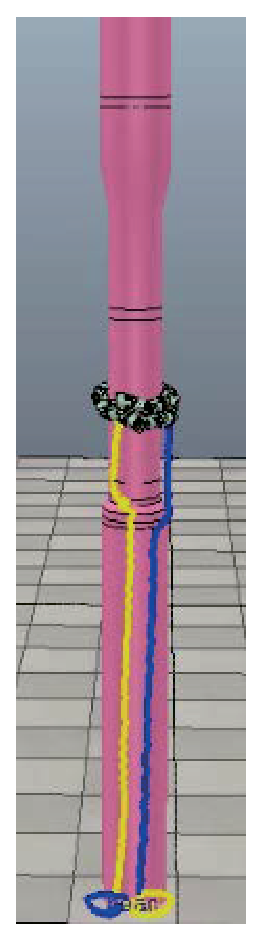
\includegraphics[height=2in,width=.12\textwidth]{fig/experiment/BSB/1m17s}
	}
	\subfigure[t=63s]{
		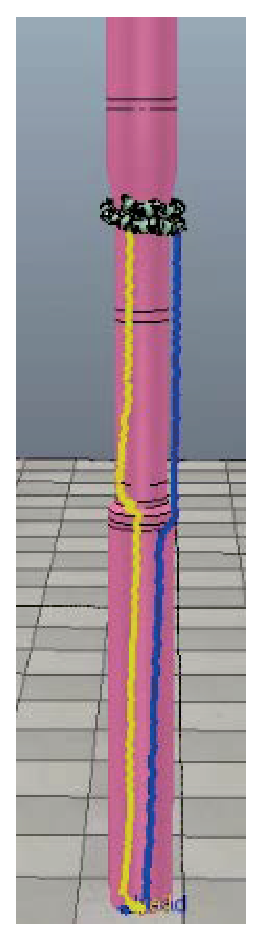
\includegraphics[height=2in,width=.12\textwidth]{fig/experiment/BSB/1m27s}
	}
	\subfigure[t=69s]{
		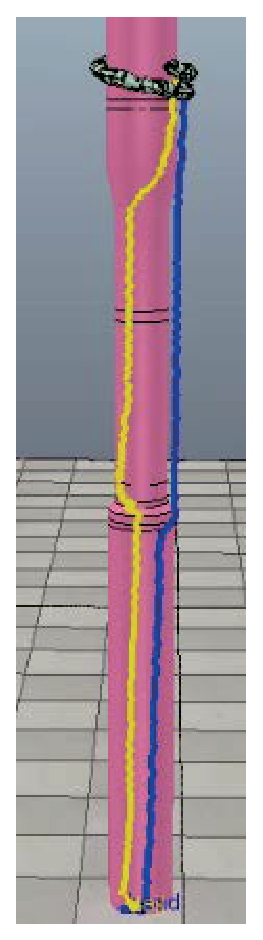
\includegraphics[height=2in,width=.12\textwidth]{fig/experiment/BSB/1m35s}
	}
	
	\subfigure[Amplitude versus Time]{
		\includegraphics[width=114pt,height=95pt]{fig/experiment/BSB/a}
		\figlabel{fig:bsa}
	}
	\subfigure[Phase versus Time]{
		\includegraphics[width=114pt,height=95pt]{fig/experiment/BSB/p}
		\figlabel{fig:bsp}
	}
	
	\subfigure[Angular rate versus Time]{
		\includegraphics[width=114pt,height=95pt]{fig/experiment/BSB/w}
		\figlabel{fig:bsw}
	}
	\subfigure[velocity versus Time]{
		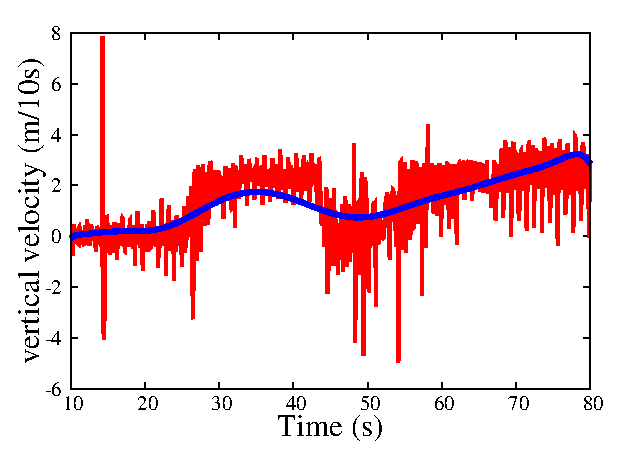
\includegraphics[width=114pt,height=95pt]{fig/experiment/BSB/v}
		\figlabel{fig:bsv}
	}
	\caption{Figure (a) to (f) is the climbing process of the snake-liked robot. Figure (g) to (j) is the parameters curve and velocity curve in climbing.}
	\figlabel{fig:BSB}
\end{figure}
We build a complex pole for simulation in this part. The pole is divided into three sections. The lowest part and the highest part are poles with 35\,cm diameter and the middle part is a pole with 25\,cm diameter. We record the parametes and the velocity during the climbing in 80 seconds.

Results are shown as \figref{fig:BSB}. From 0\,s to 24\,s, the robot changes its shape to  adapt to the unknown pipe. So in this phase, its velocity is close to zero. From 24\,s to 45\,s, the robot climbs along the part with 35\,cm diameter. In this phase, $A$, $\varepsilon$ and $\omega$ are all changing and $A$ and $\varepsilon$ are stable finally. When about 45\,s, the robot reaches the interface where the diameter changes. As the diameter changes obviously, the robot can not grasp the middle part immediately, which causes the velocity of the robot fluctuate around zero. The robot autonomously adjusts its parameters by our strategy to continue its climbing motion. From the \figref{fig:bsa}, \figref{fig:bsp} and \figref{fig:bsw}, it can be found that the parameters are increasing in this phase, which makes the robot continue moving up. Similarly, when about 63\,s, the robot meets the second interface between the middle part and the highest part. The robot maintains its motion by autonomously changing the parameters. And when the robot arrives at the highest part, all the parameters are stable at last. As a whole, the velocity changes toward bigger velocity during the motion.

Eventually all control parameters as well as velocity are stable. It shows that under this control strategy, the robot can adjust its parameters autonomously to adapt to the environment.
%\subsubsection{Simulation about climbing the pipe with 35cm lower diameter and 25cm upper diameter}

%The results are shown in \figref{fig:ccurve1}. From 0s to 15s, the robot change its shape to  adapt to the unknown pipe. So in this phase, its velocity is close to zero. From 15s to 40s, the robot climb along the pipe with 35cm diameter. In this phase, amplitude $A$, phase $\varepsilon$ and angular rate $\omega$ are all increasing and all of the them will be stable finally. About 50s, the robot reach the interface where the diameter changes. As the pipe changes obvious, the robot can not grasp the 25cm pipe immediately, which causes the velocity of the robot fluctuate around zero. The robot keeps learning and autonomously adjust its parameters to continue its climbing motion. From the \figref{fig:bsa} and \figref{fig:bsp}, it can be found that the amplitude and phase are increasing in this phase, which make the robot continue moving up.




%\begin{figure}[!h]
%	\centering
%	\subfigure[t= 0.0s]{
%		\includegraphics[height=2in,width=.12\textwidth]{fig/experiment/170912/sb0}
%	}
%	\subfigure[t=29.2s]{
%		\includegraphics[height=2in,width=.12\textwidth]{fig/experiment/170912/sb1}
%	}
%	\subfigure[t=40.5s]{
%		\includegraphics[height=2in,width=.12\textwidth]{fig/experiment/170912/sb2}
%	}	
%	\subfigure[t=55.0s]{
%		\includegraphics[height=2in,width=.12\textwidth]{fig/experiment/170912/sb3}
%	}
%	\subfigure[t=58.9s]{
%		\includegraphics[height=2in,width=.12\textwidth]{fig/experiment/170912/sb4}
%	}
%	\subfigure[t=66.0s]{
%		\includegraphics[height=2in,width=.12\textwidth]{fig/experiment/170912/sb5}
%	}
%	\subfigure[Amplifier versus Time]{
%		\includegraphics[width=.2\textwidth]{fig/experiment/170912/sbamplifier1}
%		\figlabel{fig:sba}
%	}
%	\subfigure[Phase versus Time]{
%		\includegraphics[width=.2\textwidth]{fig/experiment/170912/sbphase}
%		\figlabel{fig:sbp}
%	}
%	
%	\subfigure[Angular rate versus Time]{
%		\includegraphics[width=.2\textwidth]{fig/experiment/170912/sbangrate}
%		\figlabel{fig:sbw}
%	}
%	\subfigure[velocity versus Time]{
%		\includegraphics[width=.2\textwidth]{fig/experiment/170912/sbv}
%		\figlabel{fig:sbv}
%	}
%	\caption{The movement and the curves of parameters in the motion when the robot climb the pipe with 25cm lower diameter and 35cm upper diameter}
%	\figlabel{fig:ccurve2}
%\end{figure}

%\subsubsection{Simulation about the pipe with 35cm lower diameter and 25cm upper diameter}
%It is similar with the previous simulation, but the movement is different in the interface where the diameter changes. The results are shown in \figref{fig:ccurve2}. About 52s, the robot encounters the interface where the diameter changes. At this time the robot autonomously reduce amplitude slightly (\figref{fig:sba}) and then significantly increase  phase (\figref{fig:sbp}). In this way, the control strategy make the robot move itself from the 25cm part up to the 35cm part. 

The simulations show that our strategy is effective to adapt the robot to climb along the variable diameter pole.

\subsection{Contrast experiments on other straight poles}

As the unknown environment in the real world is complex and volatile, there may be differences between training environment and actual environment. Our training environments are vertical poles with 25\,cm or 35\,cm diameter. To ensure that this control strategy can be applied in real world situation, we conduct several  independent simulations on straight poles whose diameters are 20\,cm, 25\,cm, 30\,cm, 35\,cm or 40\,cm. The result of these simulations are shown in \figref{fig:scurve}. Next is the detailed analysis.

\begin{figure}[!h]
	\centering
%	\subfigure[d=20cm]{
%		\includegraphics[height=2in,width=.12\textwidth]{fig/experiment/170912/D20}
%		\figlabel{fig:D20}
%	}
%	\subfigure[d=25cm]{
%		\includegraphics[height=2in,width=.12\textwidth]{fig/experiment/170912/D25}
%		\figlabel{fig:D25}	
%	}
	
%	\subfigure[d=30cm]{
%		\includegraphics[height=2in,width=.12\textwidth]{fig/experiment/170912/D30}
%		\figlabel{fig:D30}
%	}
%	\subfigure[d=35cm]{
%		\includegraphics[height=2in,width=.12\textwidth]{fig/experiment/170912/D35}
%		\figlabel{fig:D35}
%	}
%	\subfigure[d=40cm]{
%		\includegraphics[height=2in,width=.12\textwidth]{fig/experiment/170912/D40}
%		\figlabel{fig:D40}
%	}	
	\subfigure[Amplitude versus Time]{
		\includegraphics[width=114pt,height=95pt]{fig/experiment/170912/samplifier}
		\figlabel{fig:samplifier}
	}
	\subfigure[Phase versus Time]{
		\includegraphics[width=114pt,height=95pt]{fig/experiment/170912/sphase}
		\figlabel{fig:sphase}
	}
	\subfigure[Angular rate versus Time]{
		\includegraphics[width=114pt,height=95pt]{fig/experiment/170912/sarate}
		\figlabel{fig:sarate}
	}
	\subfigure[velocity versus Time]{
		\includegraphics[width=114pt,height=95pt]{fig/experiment/170912/svel}
		\figlabel{fig:svelocity}
	}
	\caption{Curves about the robot climbing the poles with different diameters}
	\figlabel{fig:scurve}
\end{figure}

By observing the parameter curve we can find that the smaller diameter of the pole is, more time is required to adjust the parameters when the diameter gets smaller. All parameters finally reach a stable value and satisfy the requirements of movement. For the 40\,cm diameter pole, the robot is not long enough to form a single ring to wrap the pole. In this case the influence made by phase $\varepsilon$ is very weak (\figref{fig:sphase}). For the 20\,cm diameter pole, it is difficult for the robot to climb along the pole if we only increase the amplitude $A$, because a too large amplitude will cause the snake-liked robot curling up to a high degree, which is not conducive to climb. Therefore, to let the robot climb the pole with small diameters, we need to constantly adjust the phase $\varepsilon$ to meet the amplitude $A$'s corresponding requirements. By observing the variation curve of the control parameters of the pole with small diameter, we can found that the phase $\varepsilon$ and the amplitude $A$ of the robot are coordinated in the process of self-regulation (\figref{fig:samplifier})(\figref{fig:sphase}). The simulations show that the robot under our control strategy can catch the unknown pole and adjust itself to a suitable climbing state.

It is worth noting that, for all test environments, the movement velocity of the robot ultimately fluctuates within a constant range  (\figref{fig:svelocity}). The diameter of the pole only affects the velocity convergence rate. And also the control parameters of the robot will eventually become stable (\figref{fig:scurve}). This shows that the influence of the external environment to this control strategy is very weak. What's more, the robot will find the optimal parameter during its motion.

\subsection{Algorithm efficiency}
\figref{fig:CE-TS} shows the computing expense of our control strategy  and the time spent by the snake-liked robot when climbing poles with different diameters.

\begin{figure}[!h]
	\centering
	\subfigure[computing expenses in climbing]{
		\includegraphics[width=114pt,height=95pt]{fig/experiment/170912/figCE}
		\figlabel{fig:CE}
	}
	\subfigure[time spent in climbing]{
		\includegraphics[width=114pt,height=95pt]{fig/experiment/170912/TimeSpent}
		\figlabel{fig:TS}
	}
	\caption{Worst, best, and average case computation expenses and the total time spent of climbing the five meters high pole with different diameters}
	\figlabel{fig:CE-TS}
\end{figure}

We can see that the computation expenses are similar whatever the diameter of pole is, which indicates that the expense of our strategy not only stays in a negligible range but also receives little influence from the environment. Observe that more time is spent by the robot to climb a pole with smaller diameter. The reason is the snake-liked robot needs more time to fit its shape with a pole having a smaller diameter.

In conclusion, the simulations demonstrate that the adaptive control in robot's motion can be realized through our proposed framework.

\input{conclusion}

% trigger a \newpage just before the given reference
% number - used to balance the columns on the last page
% adjust value as needed - may need to be readjusted if
% the document is modified later
%\IEEEtriggeratref{8}
% The "triggered" command can be changed if desired:
%\IEEEtriggercmd{\enlargethispage{-5in}}

% references section

% can use a bibliography generated by BibTeX as a .bbl file
% BibTeX documentation can be easily obtained at:
% http://mirror.ctan.org/biblio/bibtex/contrib/doc/
% The IEEEtran BibTeX style support page is at:
% http://www.michaelshell.org/tex/ieeetran/bibtex/

\bibliographystyle{IEEEtran}
% argument is your BibTeX string definitions and bibliography database(s)
\bibliography{ref}





\end{document}
